\begin{frame}{Generics}{...und die Vererbung nochmal}
    \begin{itemize}
        \item Hauptgrund für Wildcards: Die "`eigenartige"' Vererbung bei generischen Klassen:
        \begin{itemize}
            \item Wenn \texttt{Integer} von \texttt{Number} erbt...
            \item Warum dann nicht auch \texttt{List<Integer>} von \texttt{List<Number>}?
        \end{itemize}
        \item Würde dazu führen, dass man inkompatible Typen zuweisen kann
        \begin{itemize}
            \item Zum Beispiel einen Double in eine \texttt{List<Integer>}
        \end{itemize}
    \end{itemize}
\end{frame}

\begin{frame}[fragile]{Generic-Vererbung}{Ein Gegenbeispiel}
\lstset{style=java}
\begin{lstlisting}
List<Number> ln = new List<Number>();
List<Integer> li = {7,12,42,46};
ln = li;    //li wird als Referenz übergeben!
//Hier würde man li einen Double hinzufügen:
ln.add(new Double(2.7182818284590));
\end{lstlisting}
\end{frame}

\begin{frame}{Wildcards}{Und deshalb braucht man sie}
    \begin{itemize}
        \item Durch "`ungewöhnliche"' Vererbungshierarchie von Generics benötigt
        \item Definieren einen unbekannten Typ
        \begin{itemize}
            \item Der jedoch eingeschränkt werden kann
            \item ...Wie bereits letztes mal besprochen
        \end{itemize}
        \item Verwendung als Argument von Funktionen
        \item Oder auch als Rückgabewert (Eher vermeiden)
    \end{itemize}
\end{frame}

\begin{frame}[fragile]{Wildcards}{Verwendung}
\lstset{style=java}
\begin{lstlisting}
void someFunc(List<?> in){ /* ... */ }   //OK
List<?> func(){ /* ... */ }              //OK

List<?> l1;   //OK
List<?> l2 = new ArrayList<>();   //OK
List<?> l3 = new ArrayList<?>();  //Fehler
\end{lstlisting}
\end{frame}

\begin{frame}{Upper-Bounded Wildcards}{Hoffentlich etwas klarer}
    \begin{itemize}[<+->]
        \item Einschränkung des Generics nach oben
        \item Dadurch gemeinsame Funktionalitäten, egal was übergeben wird
        \item \texttt{<?>} ist formal gesehen ein \texttt{<? extends Object>}
        \item Können jedoch nur lesend verwendet werden
        \item Warum?
        \begin{itemize}[<handout:0>]
            \item Beispiel \texttt{add(T)} auf eine \texttt{List<? extends Number>}
            \item Es gibt keinen Typ \texttt{T}, der auf alle Varianten von \texttt{<? extends Number>} passt
            \item Kurz: Wir können nicht sicherstellen, ob der Typ den wir schreiben überhaupt mit der speziellen Instanz kompatibel ist!
            \item Einzige Ausnahme: \texttt{null}
        \end{itemize}
    \end{itemize}
\end{frame}

\begin{frame}{Upper-Bounded Wildcards}{Visualisiert}
    \begin{figure}
        \centering
        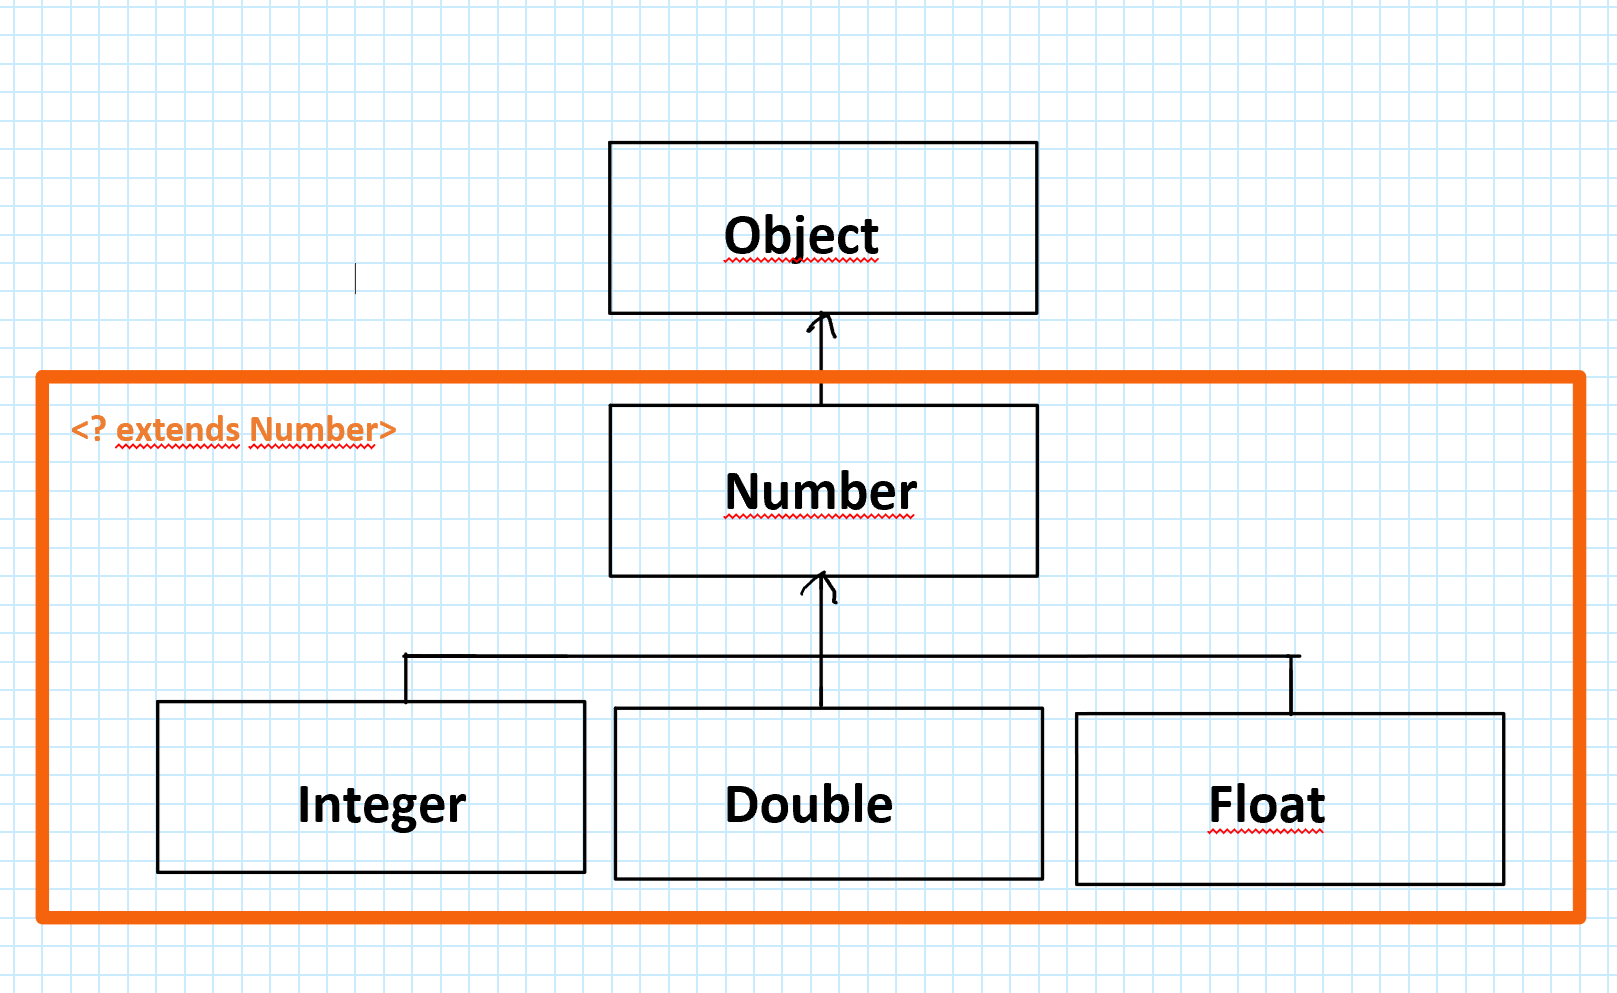
\includegraphics[height=4.5cm]{graph/wildcard_upper}
    \end{figure}
\end{frame}

\begin{frame}{Lower-Bounded Wildcards}{Nochmal erklärt}
    \begin{itemize}[<+->]
        \item Beschränken die Klasse nach unten
        \item Umgekehrter Effekt zu Upper-Bound Wildcards:
        \begin{itemize}
            \item Wir keinen lesenden Zugriff (Außer über Methoden von \texttt{Object})
            \item Dafür aber schreibeneden
            \item Dadurch keine gemeinsamen Schnittstellen
            \item Aber gemeinsamer Typ, der auf alle möglichen übergebenen Klassen passt
        \end{itemize}
        \item Frage: Welches ist dieser gemeinsame Typ? (Zum Beispiel für \texttt{List<? super Number>)}
        \begin{itemize}[<handout:0>]
            \item Immer "`unterste"' Typ (Im Sinne der Vererbung)
            \item Durch die \textbf{"`ist ein"'} Beziehung passt dieser auf alle anderen Klassen
        \end{itemize}
    \end{itemize}
\end{frame}

\begin{frame}{Lower-Bounded Wildcards}{Visualisiert}
    \begin{figure}
        \centering
        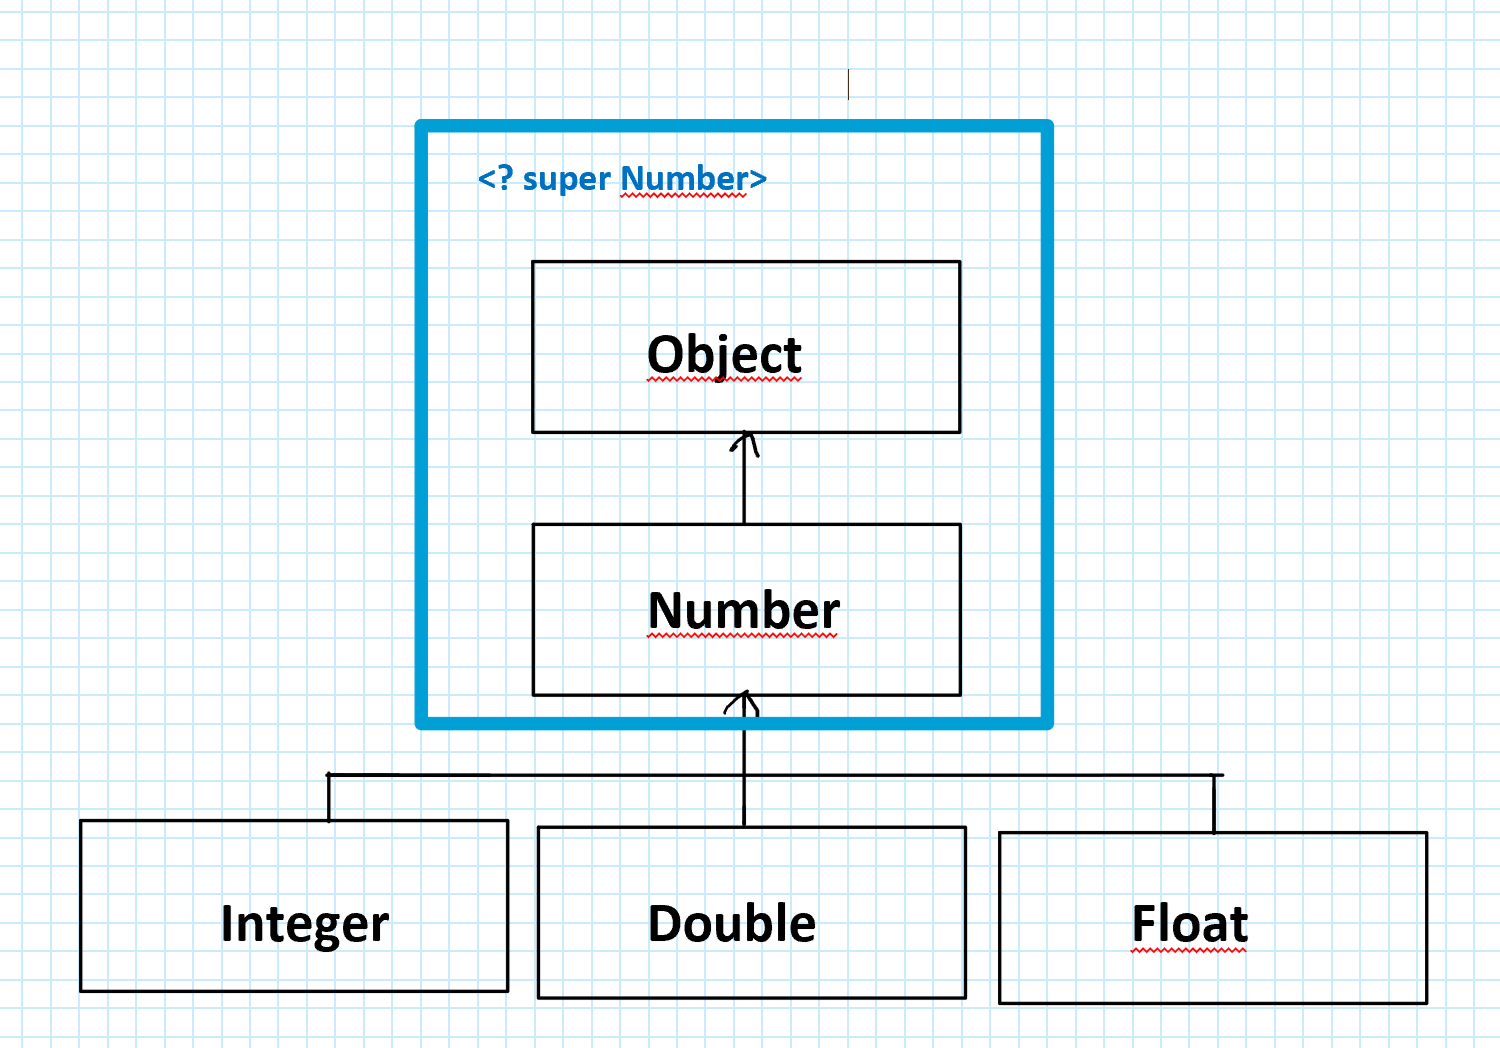
\includegraphics[height=4.5cm]{graph/lower_wildcard}
    \end{figure}
\end{frame}

\begin{frame}{Bounded Wildcards}{Nochmal in der Übersicht}
    \begin{figure}
        \centering
        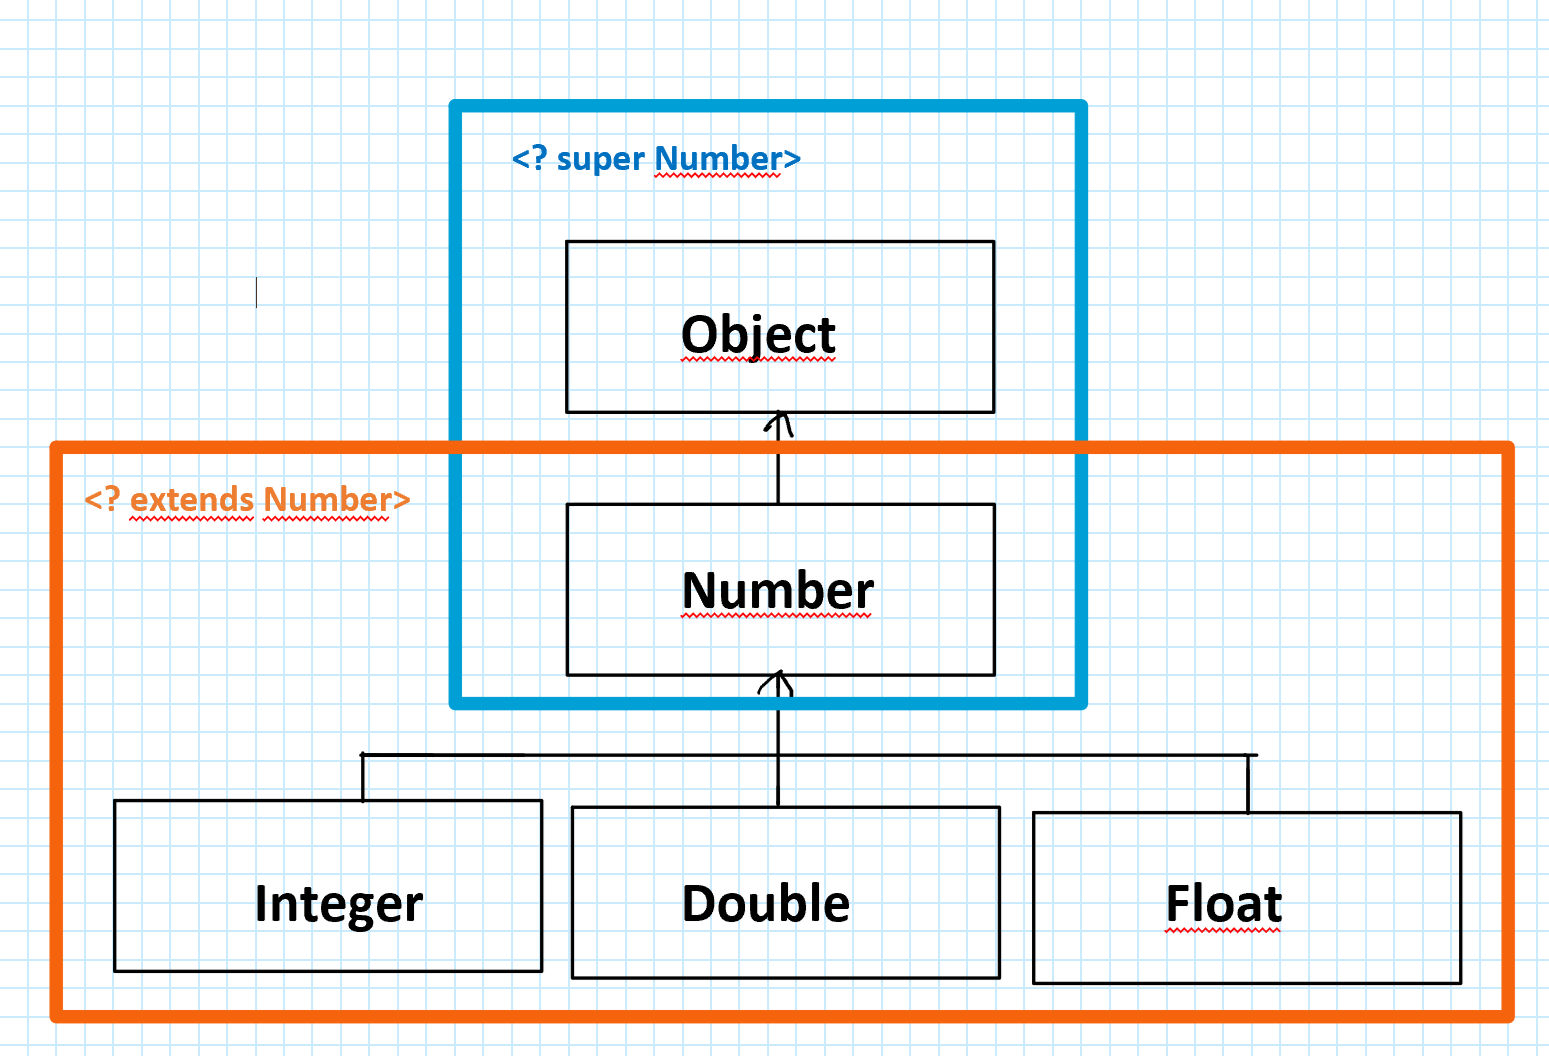
\includegraphics[height=4.5cm]{graph/wildcard_bound}
    \end{figure}
\end{frame}

\begin{frame}{Wildcards}{Und deren Vererbung}
    \begin{figure}
        \centering
        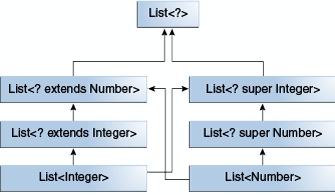
\includegraphics[height=4.5cm]{graph/generics-wildcardSubtyping}
    \end{figure}
\end{frame}